
\documentclass{beamer}
\usepackage{graphicx}

\begin{document}

\title{Probability and Statistics}
\subtitle{Understanding the Basics}
\author{DRME}
\date{\today}

\begin{frame}
  \titlepage
\end{frame}


\begin{frame}{The Set of All Possible Events}
  \begin{itemize}
    \item Overview of the concept:
      \begin{itemize}
        \item A fundamental concept in probability theory.
        \item Represents all potential outcomes or occurrences in an experiment or situation.
      \end{itemize}
    \item Significance in probability theory:
      \begin{itemize}
        \item Forms the sample space for a given experiment.
        \item Essential for defining probabilities of specific events.
      \end{itemize}
  \end{itemize}
\end{frame}

\begin{frame}{Example: Coin Toss}
  \begin{itemize}
    \item Consider the experiment of tossing a fair coin.
    \item The set of all possible events: \{Heads, Tails\}.
    \item Each outcome in the set is a possible event.
  \end{itemize}
\end{frame}

\begin{frame}{Example: Rolling a Die}
  \begin{itemize}
    \item Experiment: Rolling a six-sided die.
    \item The set of all possible events: \{1, 2, 3, 4, 5, 6\}.
    \item Each face of the die represents a possible event.
  \end{itemize}
\end{frame}

\begin{frame}{Coin Flips: Why You Should Care}
  \begin{itemize}
    \item Illustration using coin flips.
    \item Linking the concept to real-world scenarios.
  \end{itemize}
\end{frame}

\begin{frame}{Probability: Outside or Inside the Head}
  \begin{itemize}
    \item Outside the head: Long-run relative frequency.
    \item Inside the head: Subjective belief.
    \item Probabilities assign numbers to possibilities.
  \end{itemize}
\end{frame}

\begin{frame}{Outside the Head: Long-run Relative Frequency}
  \begin{itemize}
    \item Simulating a long-run relative frequency.
    \item Deriving a long-run relative frequency.
  \end{itemize}
\end{frame}

\begin{frame}{Inside the Head: Subjective Belief}
  \begin{itemize}
    \item Calibrating a subjective belief by preferences.
    \item Describing a subjective belief mathematically.
  \end{itemize}
\end{frame}

\begin{frame}{Probabilities Assign Numbers to Possibilities}
  \begin{itemize}
    \item Probabilities are assigned to different outcomes to quantify uncertainty.
    \item The assignment of probabilities is a fundamental concept in probability theory.
  \end{itemize}
\end{frame}

\begin{frame}{Understanding How Probabilities Are Assigned}
  \begin{itemize}
    \item Probabilities are numerical measures representing the likelihood of events.
    \item Assigning probabilities involves assessing the chance of different outcomes.
    \item Probabilities are expressed as values between 0 and 1, where 0 indicates impossibility, 1 indicates certainty, and values in between represent varying degrees of likelihood.
  \end{itemize}
\end{frame}

\begin{frame}{Example: Coin Toss}
  \begin{itemize}
    \item Consider a fair coin toss.
    \item There are two possible outcomes: heads (H) or tails (T).
    \item Since the coin is fair, the probability of getting heads is 0.5, and the probability of getting tails is also 0.5.
  \end{itemize}
\end{frame}

\begin{frame}{Example: Rolling a Six-sided Die}
  \begin{itemize}
    \item Suppose you roll a standard six-sided die.
    \item Each face has an equal chance of landing face up.
    \item The probability of rolling a specific number, say 3, is \( \frac{1}{6} \) because there are six possible outcomes.
  \end{itemize}
\end{frame}

\begin{frame}{Example: Drawing a Card from a Deck}
  \begin{itemize}
    \item Consider drawing a single card from a standard deck of 52 playing cards.
    \item The probability of drawing an Ace is \( \frac{4}{52} \) since there are four Aces in the deck.
    \item The probability of drawing a red card is \( \frac{26}{52} \) since half of the cards are red.
  \end{itemize}
\end{frame}



\begin{frame}{Probability Distributions}
  \begin{itemize}
    \item Overview of Probability Distributions [[see distributions.pdf]].
  \end{itemize}
\end{frame}

\begin{frame}{Discrete Distributions: Probability Mass}
  \begin{itemize}
    \item Definition: Probability mass function for discrete distributions.
    \item Examples:
      \begin{itemize}
        \item Bernoulli distribution.
        \item Binomial distribution.
        \item Poisson distribution.
      \end{itemize}
  \end{itemize}
\end{frame}

\begin{frame}{Continuous Distributions: Rendezvous with Density}
  \begin{itemize}
    \item Definition: Probability density function for continuous distributions.
    \item Examples:
      \begin{itemize}
        \item Uniform distribution.
        \item Exponential distribution.
        \item Normal distribution.
      \end{itemize}
  \end{itemize}
\end{frame}


\begin{frame}
\begin{center}
  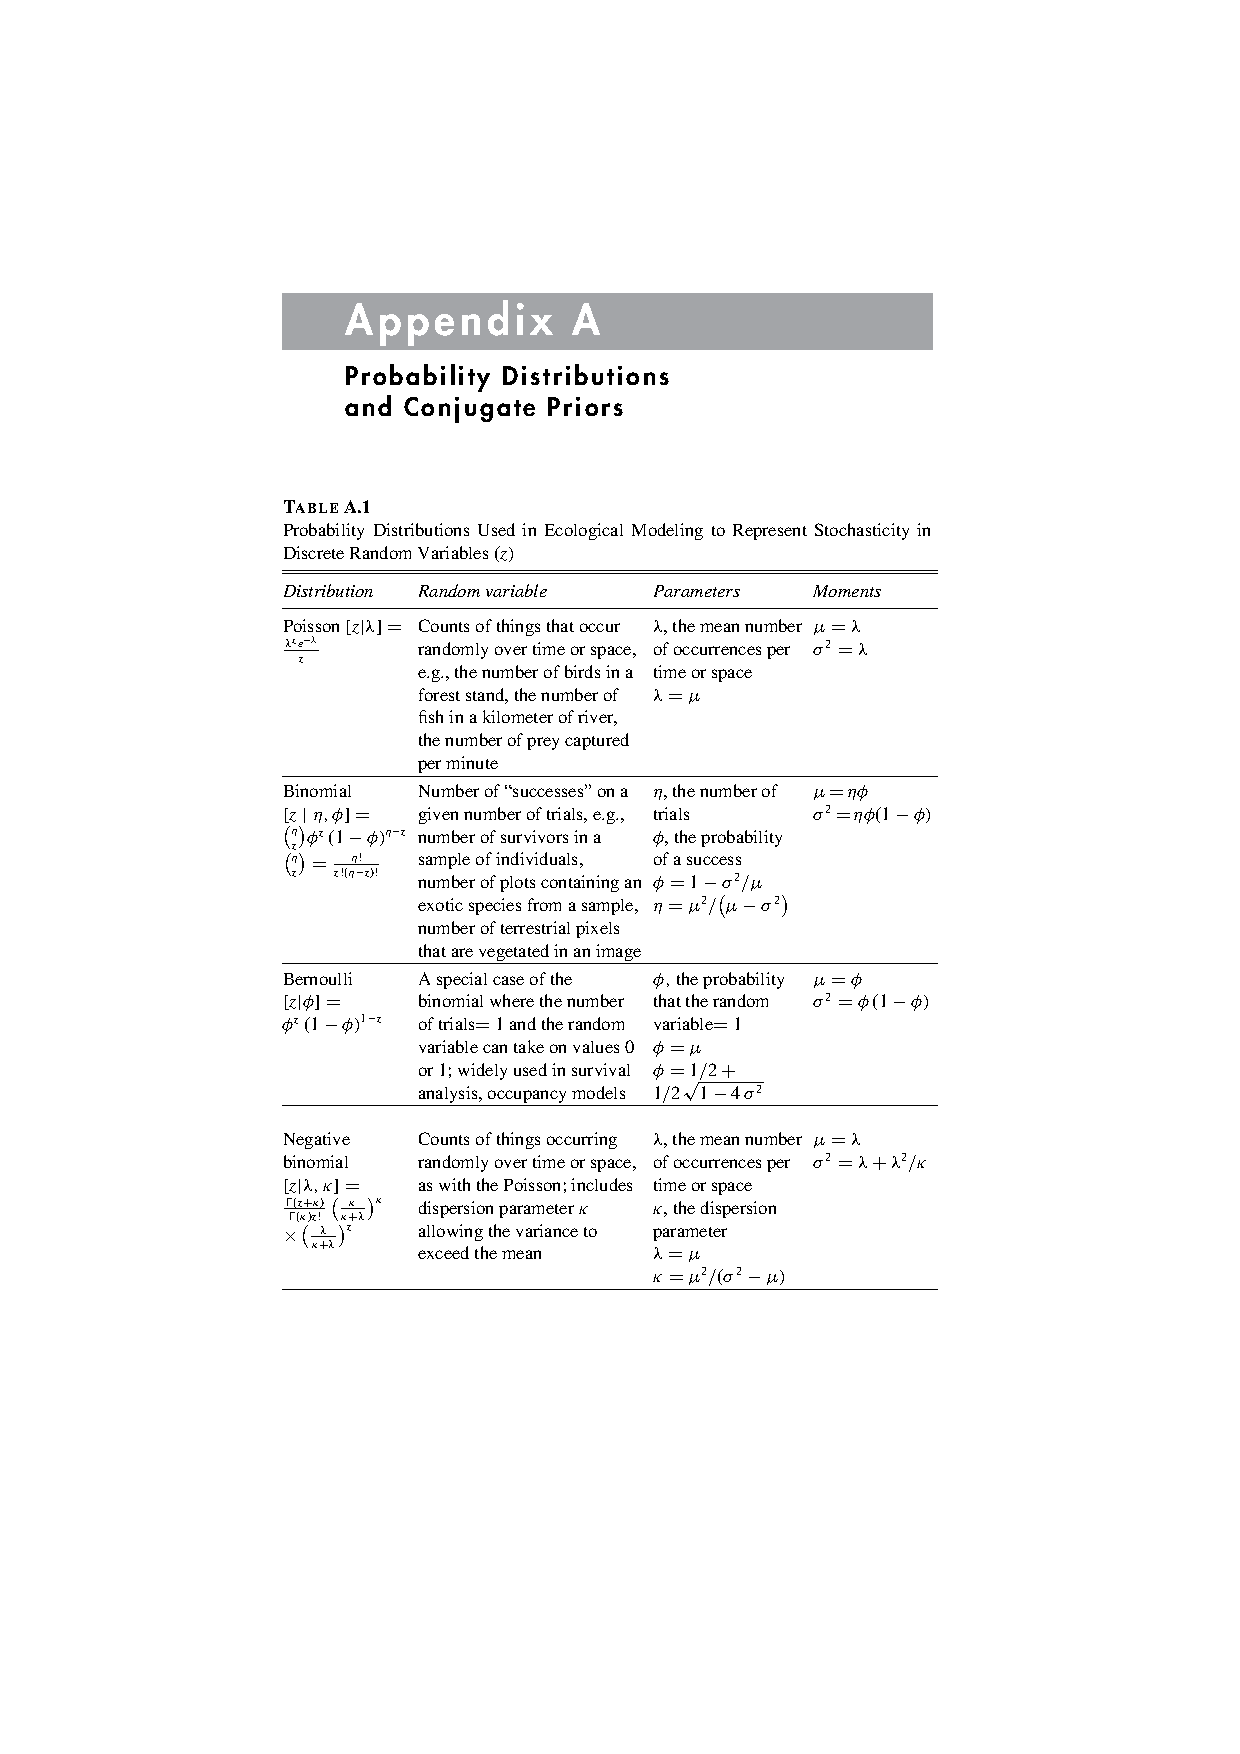
\includegraphics[page=1,width=0.65\textwidth]{distributions.pdf}
  \end{center}
\end{frame}

\begin{frame}
\begin{center}
  \includegraphics[page=2,width=0.65\textwidth]{distributions.pdf}
  \end{center}
\end{frame}

\begin{frame}
\begin{center}
  \includegraphics[page=3,width=0.65\textwidth]{distributions.pdf}
  \end{center}
\end{frame}


\begin{frame}{Properties of Probability Density Functions}
  \begin{itemize}
    \item Understanding the properties that characterize probability density functions.
    \item Emphasis on normalization and non-negativity.
  \end{itemize}
\end{frame}

\begin{frame}{The Normal Probability Density Function}
  \begin{itemize}
    \item Special focus on the normal distribution.
    \item Shape, mean, and standard deviation.
    \item Real-world examples: Height, IQ scores.
  \end{itemize}
\end{frame}



\begin{frame}{Mean and Variance of a Distribution}
  \begin{itemize}
    \item Mean as minimized variance.
  \end{itemize}
\end{frame}

\begin{frame}{Highest Density Interval (HDI)}
  \begin{itemize}
    \item Understanding the concept of HDI.
  \end{itemize}
\end{frame}

\begin{frame}{Concept of HDI}
  \begin{itemize}
    \item It provides a range of values within which a specified portion of the probability density function lies.
  \end{itemize}
\end{frame}

\begin{frame}{Why HDI Matters}
  \begin{itemize}
    \item HDI is valuable for summarizing uncertainty about a parameter.
    \item It's particularly useful when dealing with complex distributions or posterior distributions from Bayesian analysis.
  \end{itemize}
\end{frame}

\begin{frame}{Calculating HDI}
  \begin{itemize}
    \item HDI is often calculated numerically using methods such as Markov Chain Monte Carlo (MCMC).
    \item It represents the narrowest interval that contains a certain predefined probability mass.
  \end{itemize}
\end{frame}

\begin{frame}{Interpretation of HDI}
  \begin{itemize}
    \item The width of the HDI reflects the precision of our knowledge about the parameter.
    \item A narrow HDI indicates more precise estimation, while a wider HDI suggests greater uncertainty.
  \end{itemize}
\end{frame}



\begin{frame}{Two-Way Distributions}
  \begin{itemize}
    \item Conditional Probability
    \item Independence of Attributes
  \end{itemize}
\end{frame}

\begin{frame}{Conditional Probability}
  Conditional probability is the probability of an event occurring given that another event has already occurred. It is denoted by \( P(A | B) \), representing the probability of event A given that event B has occurred. The formula for conditional probability is:
  \[ P(A | B) = \frac{P(A \cap B)}{P(B)} \]
  where \( P(A \cap B) \) is the probability of both events A and B occurring, and \( P(B) \) is the probability of event B occurring.
\end{frame}

\begin{frame}{Independence of Attributes}
  Two events, A and B, are considered independent if the occurrence or non-occurrence of one event does not affect the probability of the other event. Mathematically, events A and B are independent if:
  \[ P(A \cap B) = P(A) \cdot P(B) \]
  In other words, the joint probability of A and B equals the product of their individual probabilities. If this equation holds, A and B are independent; otherwise, they are dependent.
\end{frame}


\begin{frame}{Conditional Probability}
  \begin{itemize}
    \item Conditional Probability: \( P(A | B) = \frac{P(A \cap B)}{P(B)} \)
    \item Example:
      \begin{itemize}
        \item Suppose you have a deck of cards. Let \( A \) be the event of drawing a red card, and \( B \) be the event of drawing a heart. The conditional probability of drawing a red card given that it is a heart is:
        \[ P(A | B) = \frac{P(A \cap B)}{P(B)} = \frac{\frac{1}{2}}{\frac{1}{4}} = \frac{2}{1} = 2 \]
      \end{itemize}
  \end{itemize}
\end{frame}

\begin{frame}{Independence of Attributes}
  \begin{itemize}
    \item Independence of Attributes: \( P(A \cap B) = P(A) \cdot P(B) \)
    \item Example:
      \begin{itemize}
        \item Consider two events: \( C \) is the event of rolling a 4 on a six-sided die, and \( D \) is the event of getting heads on a fair coin toss. If \( C \) and \( D \) are independent, then:
        \[ P(C \cap D) = P(C) \cdot P(D) = \frac{1}{6} \cdot \frac{1}{2} = \frac{1}{12} \]
      \end{itemize}
  \end{itemize}
\end{frame}


\begin{frame}{Joint Probability}
  \begin{itemize}
    \item Definition: The probability of the occurrence of two or more events simultaneously.
    \item Denoted as \( P(A \cap B) \) for events \( A \) and \( B \).
  \end{itemize}
\end{frame}

\begin{frame}{Joint Probability Example}
  \begin{itemize}
    \item Consider rolling a six-sided die.
    \item Let \( A \): The event of rolling an even number.
    \item Let \( B \): The event of rolling a number greater than 3.
    \item Find \( P(A \cap B) \).
  \end{itemize}
\end{frame}

\begin{frame}{Calculating Joint Probability}
  \begin{itemize}
    \item Using the formula: \( P(A \cap B) = P(A) \times P(B|A) \)
    \item \( P(A) \): Probability of event \( A \)
    \item \( P(B|A) \): Probability of event \( B \) given that event \( A \) has occurred.
  \end{itemize}
\end{frame}

\begin{frame}{Joint Probability Example}
  \begin{itemize}
    \item \( P(A) \): Probability of rolling an even number = \( \frac{3}{6} = \frac{1}{2} \)
    \item \( P(B|A) \): Probability of rolling a number greater than 3 given that an even number is rolled = \( \frac{2}{3} \)
    \item \( P(A \cap B) = \frac{1}{2} \times \frac{2}{3} = \frac{1}{3} \)
  \end{itemize}
\end{frame}

\begin{frame}{Joint Probability Interpretation}
  \begin{itemize}
    \item Joint probability provides a measure of the likelihood of multiple events occurring together.
    \item Important in understanding relationships between events.
  \end{itemize}
\end{frame}

\begin{frame}{Applications}
  \begin{itemize}
    \item Finance: Probability of a stock both gaining value and exceeding a certain threshold.
    \item Medicine: Probability of a patient having multiple symptoms simultaneously.
    \item Weather: Probability of rain and high winds occurring together.
  \end{itemize}
\end{frame}


\section{Rules of Factoring Joint Probabilities}

\begin{frame}{Rule 1: Product Rule}
  \begin{block}{Product Rule}
    \[
      P(A \cap B) = P(A|B) \cdot P(B)
    \]
    \begin{itemize}
      \item Interpretation: Probability of both events A and B occurring.
      \item or, it expresses the joint probability in terms of the conditional probability of A given B and the marginal probability of B.
    \end{itemize}
  \end{block}
\end{frame}






\begin{frame}{Rule 1: Product Rule: Example}


  \begin{itemize}
      \item Consider events A and B representing the outcomes of rolling a fair six-sided die. 
      \item Let A be the event of getting an even number (2, 4, or 6), and B be the event of getting a number greater than 3 (4, 5, or 6). 
      \item The probability of A given B is \( P(A|B) = \frac{2}{3} \), and the probability of B is \( P(B) = \frac{1}{2} \).
      \item Applying the product rule:
      
        \begin{itemize}
			\item \[ P(A \cap B) = \frac{2}{3} \cdot \frac{1}{2} = \frac{1}{3} \]
		\end{itemize}
		
   \end{itemize}

\end{frame}


\begin{frame}{Example: Genetic Inheritance}
  \begin{itemize}
    \item Event A: Offspring having a specific genetic trait.
    \item Event B: Parent carrying the gene for the trait.
    \item Using the product rule to calculate the joint probability.
  \end{itemize}
\end{frame}

\begin{frame}{Example: Species Coexistence in Ecology}
  \begin{itemize}
    \item Event A: Presence of species X in an ecosystem.
    \item Event B: Availability of a specific environmental condition.
    \item Applying the product rule to understand coexistence probabilities.
  \end{itemize}
\end{frame}



\begin{frame}{Rule 2: Chain Rule}
  \begin{block}{Chain Rule Formula}
    \[
      P(A \cap B \cap C) = P(A|B \cap C) \cdot P(B|C) \cdot P(C)
    \]
  \end{block}

  \begin{itemize}
    \item The formula for three events, generalizable to more variables.
  \end{itemize}
\end{frame}

\begin{frame}{Application in Biology}
  \begin{itemize}
    \item \textbf{Example 1: Gene Expression}
      \begin{itemize}
        \item $A$: Gene activation, $B$: Cellular environment, $C$: External signals.
        \item Probability of gene activation influenced by the cellular environment {\bf{AND}} external signals.
      \end{itemize}

    \item \textbf{Example 2: Ecosystem Dynamics}
      \begin{itemize}
        \item $A$: Predation occurrence, $B$: Prey abundance, $C$: Environmental conditions.
        \item Probability of predation depends on prey abundance  {\bf{AND}} environmental conditions.
      \end{itemize}
  \end{itemize}
\end{frame}

\begin{frame}{Generalization}
  \begin{itemize}
    \item Rule 2 can be generalized to more variables.
    \item \textbf{Example 3: Evolutionary Processes}
      \begin{itemize}
        \item $A$: Adaptation, $B$: Genetic variation, $C$: Selection pressure.
        \item Probability of adaptation influenced by genetic variation  {\bf{AND}} selection pressure.
      \end{itemize}
  \end{itemize}
\end{frame}

\begin{frame}{Rule 3: Marginalization}
  \begin{block}{Marginal Probability}
    \[
      P(A) = \sum_{B} P(A \cap B)
    \]
    Interpretation and practical implications.
  \end{block}
\end{frame}


\begin{frame}{Example: Marginalization}
  \begin{itemize}
    \item Consider a joint probability distribution table representing the occurrence of two traits in a population.
    \item Traits: Trait A (dominant/recessive) and Trait B (present/absent).
    \item Joint probabilities are given in the table.
  \end{itemize}
\end{frame}

\begin{frame}{Joint Probability Distribution Table}
  \begin{center}
    \begin{tabular}{|c|c|c|}
      \hline
      & 123 & 456 \\
      \hline
      Even  & \only<2>{1} & \only<2>{2}   \\
      \hline
      Uneven & \only<2>{2}  & \only<2>{1} \\
      \hline
    \end{tabular}
  \end{center}
\end{frame}

\begin{frame}{Joint Probability Distribution Table}
  \begin{center}
    \begin{tabular}{|c|c|c|}
      \hline
      & Trait B Present & Trait B Absent \\
      \hline
      Trait A Dominant & $P(A, B)$ & $P(A, \neg B)$ \\
      \hline
      Trait A Recessive & $P(\neg A, B)$ & $P(\neg A, \neg B)$ \\
      \hline
    \end{tabular}
  \end{center}
\end{frame}

\begin{frame}{Calculation of Marginal Probabilities}
  \begin{itemize}
    \item Marginal probability of Trait A: $P(A) = P(A, B) + P(A, \neg B)$
    \item Marginal probability of Trait B: $P(B) = P(A, B) + P(\neg A, B)$
  \end{itemize}
\end{frame}

\begin{frame}{Calculation of Marginal Probabilities}
  \begin{itemize}
    \item TABLE 3.1 [[@hobbs2015]]
  \end{itemize}
\end{frame}

\begin{frame}{Interpretation}
  \begin{itemize}
    \item Marginalization allows us to analyze the probability of individual traits independently.
    \item This is crucial for understanding the genetic composition of a population.
  \end{itemize}
\end{frame}


\end{document}
